\chapter{Equations of Lines and Planes}

\section{Lines}

A line $L$ in three-dimensional space is determined when we know a point $P_0(x_0, y_0, z_0)$ on $L$ and a direction for $L$, which is conveniently described by a vector $\vec{v}$ parallel to the line.

Let $P(x, y, z)$ be an arbitrary point on $L$ and let $\vec{r_0}$ and $\vec{r}$ be the position vectors of $P_0$ and $P$. At this moment, $\vec{r_0}$ and $\vec{r}$ have representations $\vec{OP_0}$ and $\vec{OP}$, respectively. Thus, $\vec{r} = \vec{r_0} + \vec{a}$

\begin{figure}
    \centering
    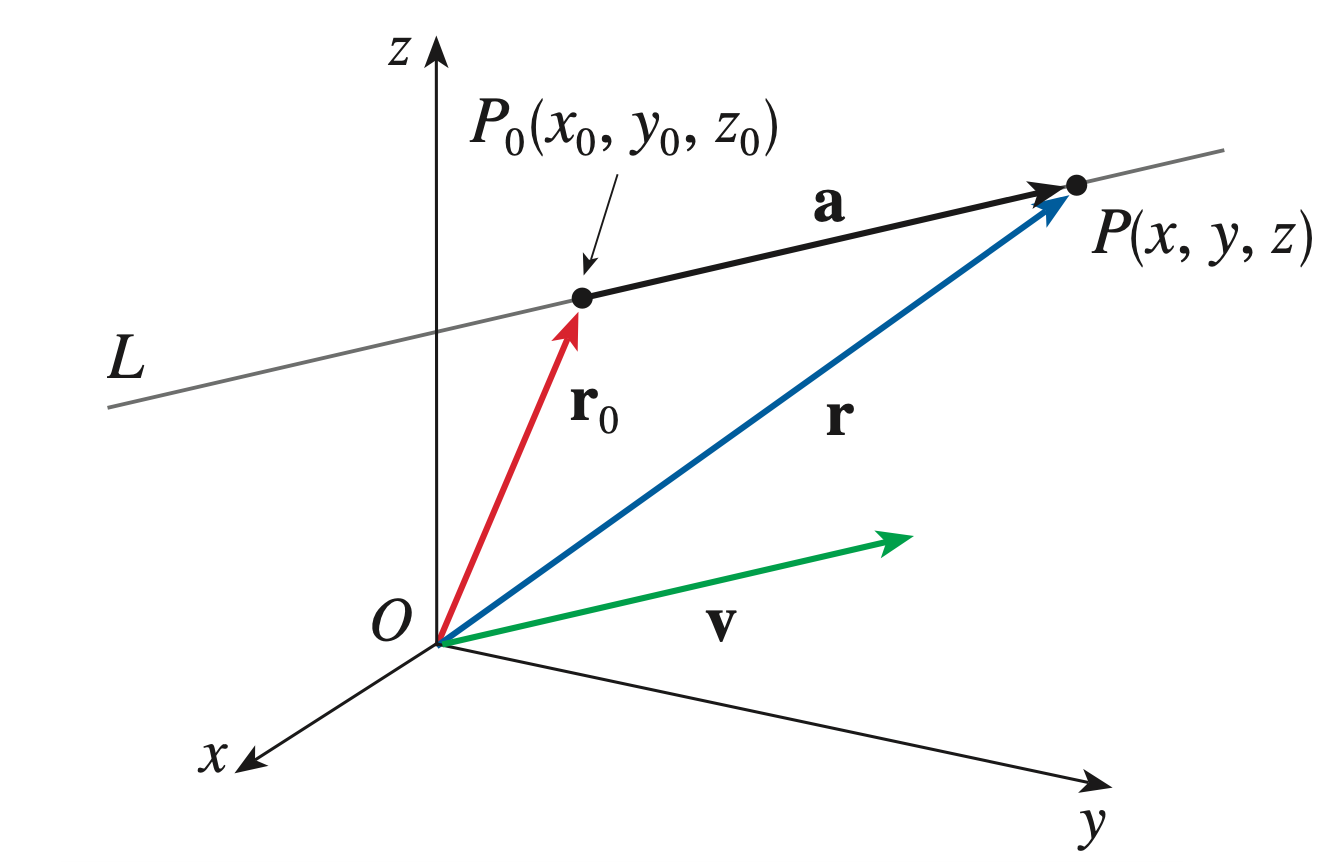
\includegraphics[width=8cm]{appendices/figures/fig003.png}
    \caption{Line representation}
\end{figure}

In the following figure, we have $\vec{v}$ is paralleled to $\vec{a}$, then $\vec{a} = t\vec{v}$. Thus, $\vec{r} = \vec{r_0} + t\vec{v}$ which is a \textbf{vector equation} of L. Each value of the parameter t gives the position vector $\vec{r}$ of a point on $L$.

\begin{figure}
    \centering
    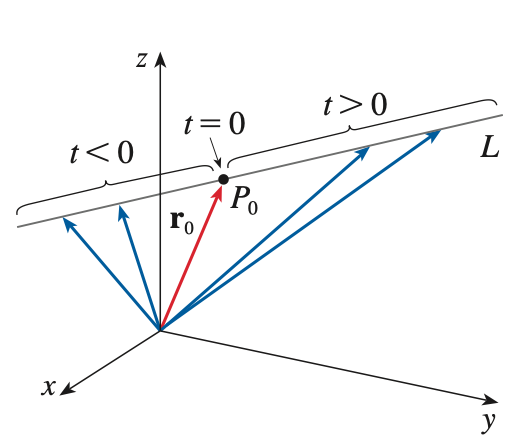
\includegraphics[width=8cm]{appendices/figures/fig004.png}
    \caption{Line representation}
\end{figure}

Given $v = <a, b, c>$, $r=<x, y, z>$ and $r_0=<x_0, y_0, z_0>$, then

\begin{equation}
    <x, y, z> = <x_0 + ta, y_0 + tb, z_0 + tc>
\end{equation}

Two vectors are equal if and only if corresponding components are equal. Therefore, we have three scalar equations:

\begin{equation}
    \label{parametric equation}
  \left\{
    \begin{aligned}
      & x = x_0 + ta\\
      & y = y_0 + tb\\
      & z = z_0 + tc
    \end{aligned}
  \right.
\end{equation}

where $t \in \mathbb{R}$.

These equations are called \textbf{parametric equations} of the line L through the point $P_0(x_0, y_0, z_0)$ and parallel to the vector $\vec{v} = <a, b, c>$. Each value of $t$ gives a point $(x, y, z)$ on $L$.

From the \ref{parametric equation} we have,

\begin{equation}
    \label{symmetric equation}
    \frac{x - x_0}{a} = \frac{y - y_0}{b} = \frac{z - z_0}{c}
\end{equation}

If the line pass through one more point $r_1$, then $\vec{v} = r_1 - r_0$ and

\begin{equation}
    r = r_0 + t(r_1 - r_0) = (1 - t)r_0 + tr_1
\end{equation}


\section{Planes}

A single vector parallel to the plane is not enough to convey the "direction" of the plane, but a vector perpendicular to the planes does completely specify its direction. Thus a plane is space is determined by a point $P_0(x_0, y_0, z_0)$ in the plane and a vector $\vec{n}$ that is orthogonal to the plane. This orthogonal vector $\vec{n}$ is called a \textbf{normal vector}.

Let $P(x, y, z)$ be an arbitrary point the plane, and let $\vec{r_0}$ and $\vec{r}$ be the position vectors of $P_0$ and $P$. Then the vector $\vec{r} - \vec{r_0}$ is represented by $\vec{P_0P}$

The normal vector $\vec{n}$ is orthogonal to every vector in the given plane. In particular, $\vec{n}$ is orthogonal to $\vec{r} - \vec{r_0}$ and so we have

\begin{figure}
    \centering
    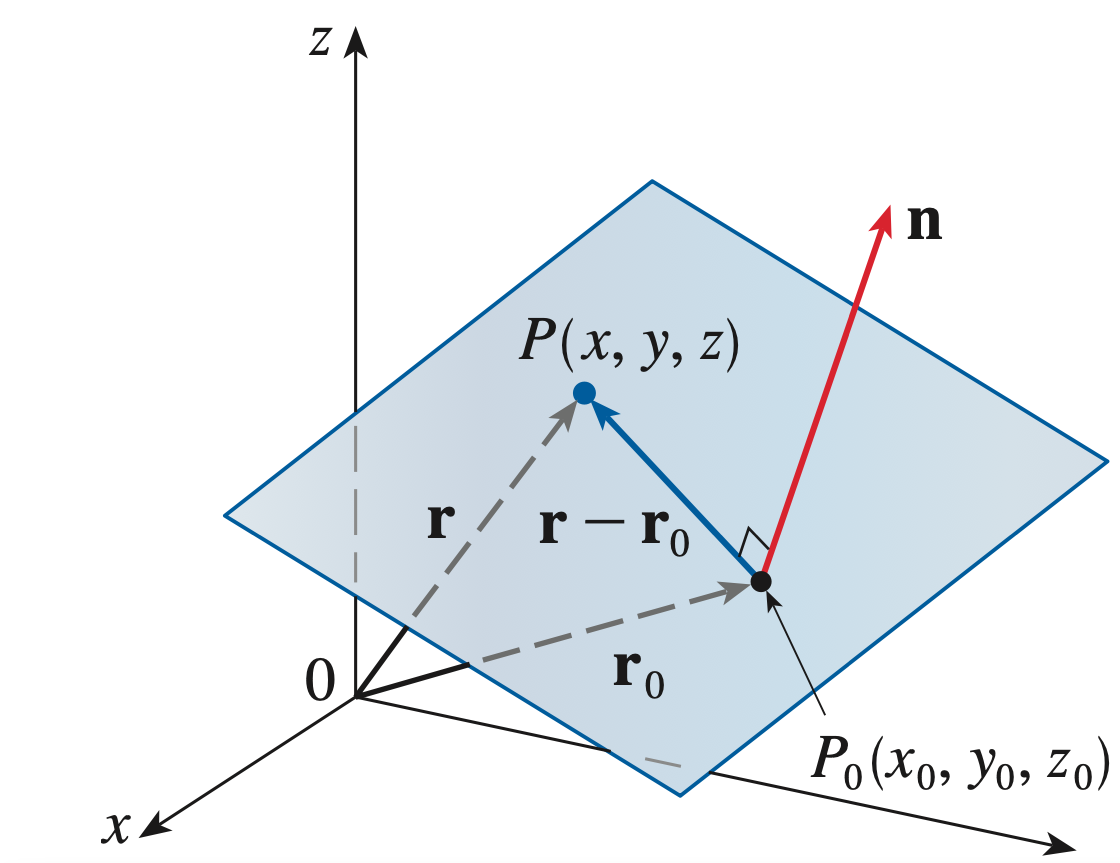
\includegraphics[width=8cm]{appendices/figures/fig005}
    \caption{Line representation}
\end{figure}

\begin{equation}
    \label{Vector equation of a plane}
    n \cdot (\vec{r} - \vec{r_0}) = 0 \Leftrightarrow n \cdot r = n \cdot r_0
\end{equation}

\ref{Vector equation of a plane} is called \textbf{Vector equation of a plane}.

Given $n = <a, b, c>, r = <x, y, z>$ and $r_0 = <x_0, y_0, z_0>$, then

\begin{equation}
    <a, b, c> \cdot <x - x_0, y - y_0, z - z_0> = 0
\end{equation}

In other words,

\begin{equation}
    \label{Linear equation of the plane}
    \begin{split}
        a(x - x_0) + b(y - y_0) + c(z - z_0) & = 0\\
        \Leftrightarrow ax - ax_0 + by - by_0 + cz - cz_0 & = 0\\
        \Leftrightarrow ax + by + cz - ax_0 - by_0 - cz_0 & = 0\\
        \Leftrightarrow ax + by + cz + d = 0
    \end{split}
\end{equation}

where $d = -(ax_0 + by_0 + cz_0)$ 

\ref{Linear equation of the plane} is called a \textbf{linear equation}.

In machine learning, we usually,

\begin{align}
    w &= \begin{bmatrix}
           a \\
           b \\
           c
         \end{bmatrix}
\end{align}

and

\begin{align}
    x &= \begin{bmatrix}
           x_1 \\
           x_2 \\
           x_3
         \end{bmatrix}
  \end{align}

where $x$ is a data point and $x_1, x_2$ and $x_3$ is its vector components. Then, \ref{Linear equation of the plane} is represented as

\begin{equation}
    w^Tx + d = 0    
\end{equation}

Thus, $w$ is \textbf{normal vector} of the plane.

\section{Distance}

In order to find a formula for the distance $D$ from a point $P_1(x_1, y_1, z_1)$ to the plane $ax + by + cz + d = 0$, we let $P_0(x_0, y_0, z_0)$ be any point in the given plane and $\vec{b}$ be the vector corresponding to $\vec{P_0P_1}$. Then,

\begin{equation}
    b = <x_1 - x_0, y_1 - y_0, z_1 - z_0>
\end{equation}

the distance $D$ from $P_1$ to the plane is equal to the absolute value of the scalar projection of $\vec{b}$ onto the normal vector $\vec{n} = <a, b, c>$. Thus,

\begin{equation}
    \begin{split}
        D & = ||comp_n\vec{b}|\\
          & = \frac{|n \cdot b|}{|n|}\\
          & = \frac{|a(x_1 - x_0) + b(y_1 - y_0) + c(z_1 - z_0)|}{\sqrt{a^2 + b^2 + c^2}}\\
          & = \frac{|ax_1 + by_1 + cz_1 + d|}{\sqrt{a^2 + b^2 + c^2}}
    \end{split}
\end{equation}

